\section{Ingestion-Service}

Der Ingestion-Service hat die Aufgabe eine Ingestion für eine Datenquelle durchzuführen.
Dazu gehören das Laden der Daten in ein DataFrame, die Deltaberechnung und das Speichern.
Das meiste davon wird jedoch nicht von dem Service selbst, sondern auf dem Spark Cluster gemacht.
Der Service führt die Vorbereitung und das Deplyoment des Jobs auf dem Cluster aus.

Der Ingestion-Service wartet auf Nachrichten zur Ausführung einer Ingestion, mit der Id der DataSourceDefinition.
Für jede Nachricht wird ein neuer Prozess gestartet, der die Komplette Ausführung der Ingestion übernimmt.
Auf diese Art können mehrer Ingestion von verschiedenen Quellen parallel bearbeitet werden.

Der Ablauf einer einzelnen Ingestion kann unabhängig vom Ingestion- oder Speicher-Typ in einem allgemeinen Ablauf abgebildet werden.
Als erstes wird geprüft, ob eine Ingestion asugeführt werden darf, also ob für diese Datenquelle bereits eine Ingestion läuft.
Danach kommt die Vorbereitung.
Hier werden die Plugins installiert und eine SparkSession erstellt.
Im nächsten Schritt werden die Daten aus der Quelle in ein DataFrame geladen.
Darauf folgt eine Entscheidung, ob eine Deltaberechnung durchgeführt werden muss.
Es gelten diese Bedingungen: \begin{itemize}
    \item der Speicher-Typ ist Delta
    \item es handelt sich nicht um eine Updatequelle
    \item es ist nicht die erste Ingestion dieser Datenquelle
\end{itemize}
Sind alle davon erfüllt, werden Änderungsdaten zwischen dem geladenen DataFrame und den aktuellen Daten aus dem Data Lake berechnet.
Wurden Änderungsdaten berechnet oder handelt es sich um eine Updatequelle, werden diese in die Daten der entsprechenden Datenquelle eingepflegt.
Ansonsten werden die Daten einfach geschrieben.
Handelt es sich nicht um einen benutzerdefinierten Speicher, werden die alten Daten mit den neuen überschrieben.

\begin{figure}
    \centering
    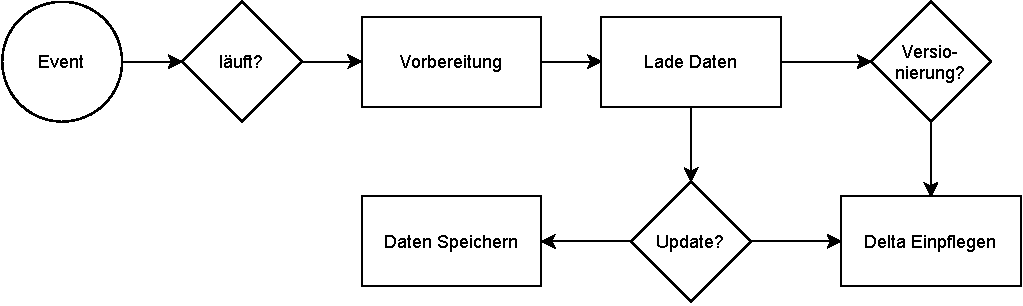
\includegraphics[width=\textwidth]{Grafiken/Entwicklung-Ingestion-Ablauf.pdf}
    \caption{Allgemeiner Ablauf einer Ingestion}
    \label{fig:ingestion-ablauf}
\end{figure}